\documentclass[journal,12pt,twocolumn]{IEEEtran}
\usepackage{graphicx}
\usepackage[cmex10]{amsmath}
\usepackage[margin=0.5in]{geometry}
\graphicspath{{./figs/}}{}
\usepackage{amsmath,amssymb,amsfonts,amsthm}
\newcommand{\myvec}[1]{\ensuremath{\begin{pmatrix}#1\end{pmatrix}}}
\usepackage{listings}
\usepackage{watermark}
\usepackage{array}
\usepackage{booktabs}
\usepackage{mathtools}
\usepackage{titlesec}
\usepackage[thinc]{esdiff}
\let\vec\mathbf
\lstset{
frame=single, 
breaklines=true,
columns=fullflexible
}
%\thiswatermark{\centering \put(0,-105.0){\includegraphics[scale=0.5]{iith.png}} }

\title{\mytitle}
\title
{ Optimisation Assignment 
}
\author{Adarsh Kumar (FWC22068)}
\begin{document}
\maketitle
\tableofcontents
\bigskip


\section{Problem}
If the function $ f(x) = 2x^3 -9ax^2+ 12a^2x+1 $, where $a > 0$ , attains its maximum and minimum at p and q respectively. Such that $ p^2 =q$ ,then a equals?
\linebreak
A) $\frac{1}{2}$ \hspace{2mm} B) 3\hspace{2mm}  C) 1  \hspace{2mm}D) 2\hspace{2mm}
\\
\section{Figure}
\begin{figure}[h]
    \centering
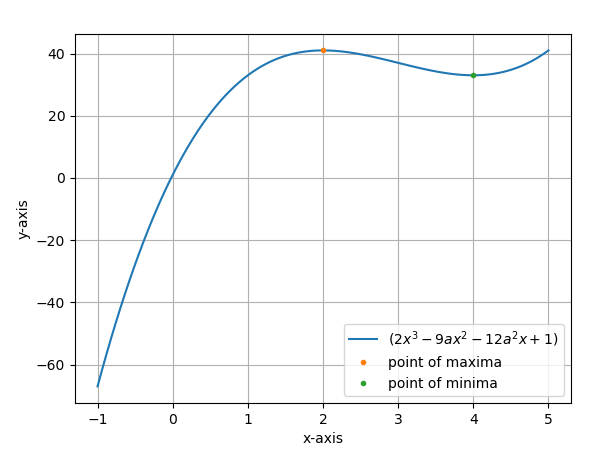
\includegraphics[width=\columnwidth]{opt.png}
    \label{fig:my_label}
\end{figure}

\section{Solution}
Assume a=2 ,\\
Given p is maxima point and q is minima point\\

So., we can write the given equation as: 
\begin{align}
 f(x) = 2x^3 -18x^2+ 48x+1
\end{align} 
we can find the maxima of eq(1) by using gradient ascent method
	\begin{align}
	 x_{n+1} &= x_n + \alpha \nabla f(x_n) 
	\end{align}
	\begin{align}
	 x_{n+1} &= x_n + \alpha (6x^2 - 36x + 48)
	\end{align}
Taking $x_0=0.5,\alpha=0.001$ and precision = 0.00000001, values obtained using python are:
    
    \begin{align}
        \boxed{\text{Maxima} = 40.99999999999584 \approx 41}\\
        \boxed{\text{Maxima Point} =1.9999991677483622 \approx 2}
    \end{align}
  Now,\\ 
   we can find the minima of eq(1) by using gradient descent method
 
$\implies x_{n+1} = x_n - \alpha \nabla f(x_n) $\\
 \begin{align}
  x_{n+1} &= x_n - \alpha (6x^2 - 36x + 48)
    \end{align}\\
Taking $x_0=3.5,\alpha=0.001$ and precision = 0.00000001, values obtained using python are:
    
    \begin{align}
        \boxed{\text{Minima} =33.00000000000418 \approx 33}\\
        \boxed{\text{Minima Point} = 3.9999991682037273 \approx 4}
    \end{align}
\\
so here we have calculated ,\\
Maxima point i.e $p = 2$\\
And , Minima $q =4$

which satisfies the condition $p^2 = q$
\\
Hence $a=2$ , option D is the correct answer. \\
\begin{lstlisting}
https://github.com/aadrshptel/Fwc_module1/tree/main/Assignments/Matrix%20assignments/Optimisation/codes
\end{lstlisting}
Execute the code by using the command\\
\textbf{python3 opt.py}
\end{document}